\section{First Dark Matter Results from the Commissioning Run}
\label{secRun07}

First dark matter search results have been obtained using 11.17 live days of data acquired in the commissioning run in October and November 2009, prior to the calibration with an $^{241}$Am-Be neutron source. The acceptance corrected exposure, weighted by the energy spectrum of a 100~GeV/c$^{2}$ WIMP, is 172~kg$\cdot$days. Although the data has not been `blinded', all analysis cuts and event selection criteria have been defined only on the calibration data.

The energy region for the WIMP-search has been chosen between 4~PE and 20~PE, which corresponds to the nuclear recoil equivalent energy 8.7$-$32.6~keV$_{\mathrm{nr}}$, defined based on the $L_{eff}$ parameterization described in Section~\ref{secLeff}. 
%, and taking into account the S1 resolution dominated by Poisson fluctuations. 
The lower bound is motivated by the acceptance of the PMT coincidence level requirement, which had been determined with a Monte Carlo simulation as $>$90\% at 4~PE. The upper bound is is chosen to approximately correspond to the one used in the XENON10 analysis~\cite{xe10-independent}.

Electronic and nuclear recoil bands have been calibrated with $^{60}$Co and $^{241}$Am-Be sources, respectively. For details, see Section~\ref{secBandCalibration}. 
A lower threshold for the S2 signal has been set at 300~PE, which corresponds to about 15 ionization electrons. The signal region has been defined above this threshold, and below the median of the nuclear recoil band (see Section~\ref{secBandCalibration}), thus resulting in an energy-independent signal acceptance of 50\% (Fig.~\ref{figCutsAcceptance}). The corresponding electronic recoil discrimination is $>$99\%, which results in a predicted background of $<$0.2 events in this WIMP-search region for 11.17~days and 40~kg fiducial mass.

\begin{figure}[!h]
\centering
\subfigure[]{
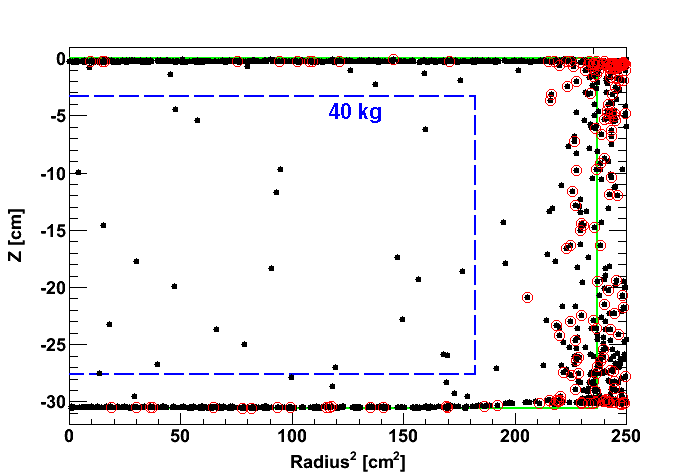
\includegraphics[width=0.475\linewidth]{plots/run07/run07_RZ_mod_withLabels.png}
\label{figRun07log10_1}}
\subfigure[]{
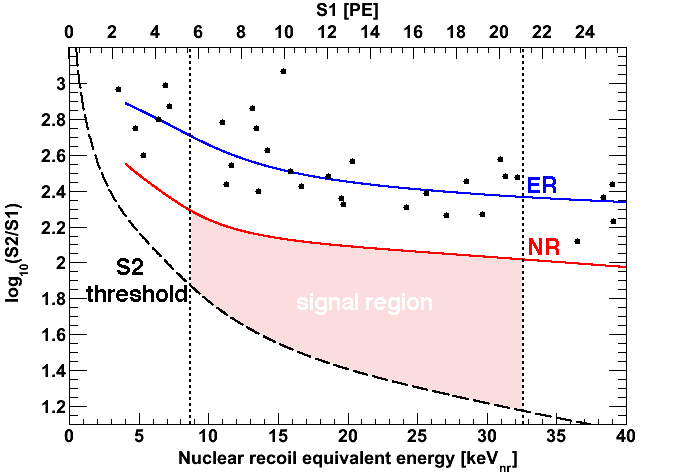
\includegraphics[width=0.475\linewidth]{plots/run07/run07_log10_mod_withContourAndLabels1.png}
\label{figRun07log10_2}}
\caption[Spatial distribution of events observed in the commissioning run (run07 and discrimination parameter log$_{10}$(S2/S1) as a function of the nuclear recoil energy)]{
 (a) - distribution of all events in the 11.17 live days of the commissioning run in 2009 (run07) in the energy range 8.7-32.6~keV$_{\mathrm{nr}}$ (black markers), and events  in the signal region (red circles). The 40~kg fiducial volume is shown by the blue dashed lines, the green lines indicate the physical dimensions of the liquid xenon target volume. 
(b) - discrimination parameter log$_{10}$(S2/S1) as a function of the deposited energy for events in the 40~kg fiducial volume. The median of the electronic recoil band is shown by the blue line, the red line shows the median of the nuclear recoil band. The vertical dashed lines indicate the WIMP-search energy region. All 22 interactions in the 40~kg fiducial volume are in the electronic recoil band.
No events below the nuclear recoil median have been observed. 
Figures published in Ref.~\cite{xe100-run08}.}
\label{figRun07log10}
\end{figure}

\begin{figure}[!b]
\centering
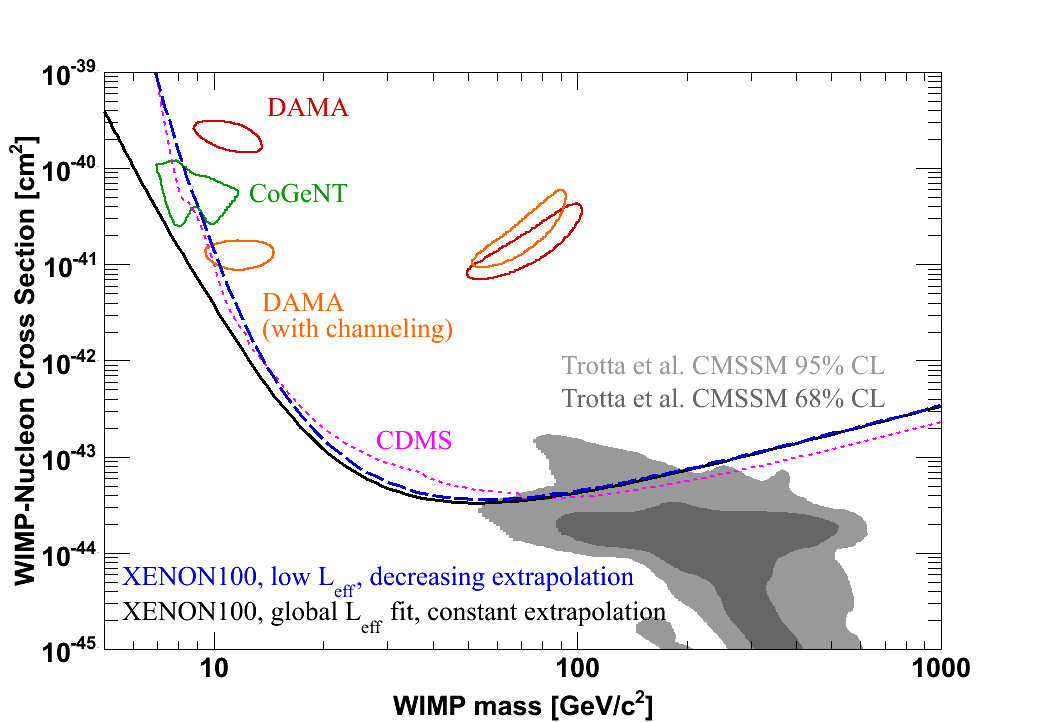
\includegraphics[width=0.6\linewidth]{plots/run07/run07_limit_mod.png}
\caption[The first XENON100 exclusion limit on the spin-independent elastic scattering WIMP-nucleon cross section]{The 90\% confidence limit on the spin-independent elastic scattering WIMP-nucleon cross section (black and blue lines), together with the expectations from a theoretical model~\cite{Yellin}. Also shown are the limit from CDMS (dotted magenta line)~\cite{CDMS_limit}, and the areas at 90\% confidence level favored by DAMA (dark red - without channeling, dark red - with channeling) and CoGeNT (green contour). Figure published in Ref.~\cite{xe100-run07}.}
\label{figRun07limit}
\end{figure}

A fiducial mass of 40~kg has been chosen for the analysis, defined as a cylinder with 13.5~cm radius  and 24.3~cm height. The spatial distribution of single scatter events observed the data is shown in Fig.~\ref{figRun07log10_1}. The observed high density of events outside of the physical radius of the TPC (15.3~mm) is due to systematic effect of the SVM position reconstruction algorithm used for the analysis~(see Fig.~\ref{figPosRecCo60}). All 22 interactions in the target volume are crearly in the electronic recoil band, none of these being in the pre-defined signal region (Fig.~\ref{figRun07log10_2}). The observed rate and the flat spectrum agree well with the predictions from the Monte Carlo simulations with GEANT4, described in Chapter~\ref{chERbackground}. 

An upper limit on the spin-independent WIMP-nucleon elastic scattering cross section has been derived from the observation based on the assumption of an isothermal WIMP halo with a local circular velocity of 220~km/s, a density of 0.3~GeV/c$^{2}$, and an escape velocity of 544~km/s~\cite{LewinSmith, Smith}. The resulting 90\% confidence upper limit on spin-independent cross section is shown in Fig.~\ref{figRun07limit}. The minimum is at 3.4$\times$10$^{-44}$~cm$^{2}$ for a WIMP mass of 55~GeV/c$^{2}$. The impact of the nuclear recoil energy scale based on the $L_{eff}$ following the lower 90\% confidence contour, together with the extrapolation below 5~keV$_{\mathrm{nr}}$ to zero at 1~keV$_{\mathrm{nr}}$, has also been determined, and is shown in the figure. 
The sensitivity is comparable to that of the CDMS~\cite{CDMS_limit} experiment, and constraints the interpretation of the DAMA~\cite{DAMA_LightWIMP} and CoGeNT~\cite{CoGeNT_LightWIMP, CoGeNT_modulation} modulated signals as being due to light mass WIMPs. These initial result from only 11.17~live days of data crearly demonstrates the potential of the XENON100 experiment to discover dark matter.














